% ============================================================
\chapter{Homologie Persistante}
\label{ch:persistante}
% ============================================================

L'homologie classique r\'epond \`a la question~: \og combien de trous a cet espace~? \fg Mais en analyse topologique des donn\'ees, l'espace lui-m\^eme n'est pas donn\'e~: on n'a qu'un nuage de points, et la topologie d\'epend du param\`etre d'\'echelle choisi. \`A petite \'echelle, chaque point est isol\'e~; \`a grande \'echelle, tout fusionne en une seule composante connexe. La question devient alors~: \og quelles caract\'eristiques topologiques \emph{persistent} \`a travers les \'echelles~? \fg C'est l'id\'ee fondatrice de l'homologie persistante, d\'evelopp\'ee au d\'ebut des ann\'ees 2000 par Herbert Edelsbrunner, David Letscher et Afra Zomorodian, puis enrichie par Gunnar Carlsson et ses collaborateurs.

Le r\'esultat cl\'e est que la persistance peut \^etre repr\'esent\'ee par un \emph{diagramme de persistance}~: un ensemble de points dans le plan, o\`u chaque point $(b, d)$ encode la naissance et la mort d'une caract\'eristique topologique. Les points loin de la diagonale correspondent \`a des structures robustes~; ceux pr\`es de la diagonale sont du bruit. Cette repr\'esentation, \`a la fois simple et puissante, est devenue l'outil central de la TDA.

\begin{intuition}
L'homologie classique d\'ecrit la topologie d'un espace fix\'e.
L'homologie \emph{persistante} \'etudie comment cette topologie
\emph{\'evolue} lorsqu'on parcourt une famille embo\^{\i}t\'ee de
complexes~: elle d\'etecte quand une caract\'eristique topologique
na\^{\i}t, et quand elle meurt.
\end{intuition}

% ============================================================
\section{Filtrations}
% ============================================================

\begin{definition}[Filtration d'un complexe simplicial]
Une \emph{filtration} d'un complexe simplicial $K$ est une suite
croissante de sous-complexes~:
\[
  \emptyset = K_0 \subseteq K_1 \subseteq K_2 \subseteq \cdots
  \subseteq K_m = K
\]
telle que pour tout $i$, $K_i$ est un sous-complexe de $K$.
\end{definition}

\begin{definition}[Filtration par valeurs]
De mani\`ere \'equivalente, une filtration peut \^etre d\'ecrite par
une fonction $f : K \to \R$ telle que pour tout $\sigma \in K$ et
toute face $\tau \subseteq \sigma$, on a $f(\tau) \leq f(\sigma)$.
Le complexe filtr\'e au niveau $r$ est alors~:
\[
  K_r = f^{-1}((-\infty, r]) = \{\sigma \in K : f(\sigma) \leq r\}.
\]
\end{definition}

\begin{exemple}[Filtration de Vietoris--Rips]
\'Etant donn\'e un nuage de points $X \subset \R^d$, la filtration de
Vietoris--Rips est d\'efinie par~:
\[
  \mathrm{VR}(X, r) = \big\{
    \sigma \subseteq X : \norm{x_i - x_j} \leq 2r
    \;\text{pour tous}\; x_i, x_j \in \sigma
  \big\}.
\]
Lorsque $r$ cro\^{\i}t, de plus en plus de simplexes apparaissent.
\end{exemple}

\begin{center}
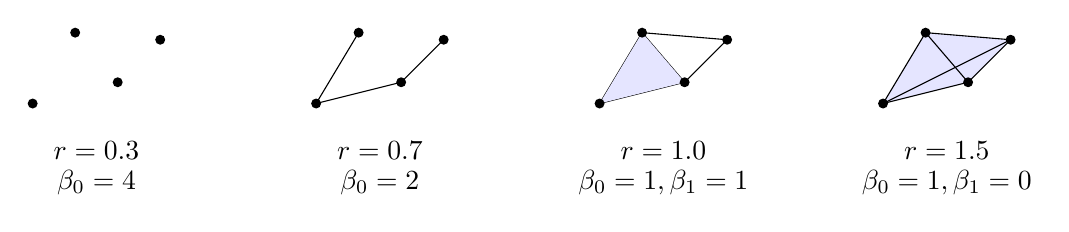
\begin{tikzpicture}[scale=0.9]
  % r = 0.3
  \begin{scope}[shift={(0,0)}]
    \foreach \p in {(0,0),(1.2,0.3),(0.6,1.0),(1.8,0.9)}{
      \fill \p circle (2pt);
    }
    \node[below] at (0.9,-0.4) {$r = 0.3$};
    \node[below] at (0.9,-0.8) {$\beta_0 = 4$};
  \end{scope}
  % r = 0.7
  \begin{scope}[shift={(4,0)}]
    \draw (0,0) -- (1.2,0.3);
    \draw (0,0) -- (0.6,1.0);
    \draw (1.2,0.3) -- (1.8,0.9);
    \foreach \p in {(0,0),(1.2,0.3),(0.6,1.0),(1.8,0.9)}{
      \fill \p circle (2pt);
    }
    \node[below] at (0.9,-0.4) {$r = 0.7$};
    \node[below] at (0.9,-0.8) {$\beta_0 = 2$};
  \end{scope}
  % r = 1.0
  \begin{scope}[shift={(8,0)}]
    \draw (0,0) -- (1.2,0.3) -- (0.6,1.0) -- cycle;
    \draw (1.2,0.3) -- (1.8,0.9) -- (0.6,1.0);
    \fill[blue!10] (0,0) -- (1.2,0.3) -- (0.6,1.0) -- cycle;
    \foreach \p in {(0,0),(1.2,0.3),(0.6,1.0),(1.8,0.9)}{
      \fill \p circle (2pt);
    }
    \node[below] at (0.9,-0.4) {$r = 1.0$};
    \node[below] at (0.9,-0.8) {$\beta_0 = 1, \beta_1 = 1$};
  \end{scope}
  % r = 1.5
  \begin{scope}[shift={(12,0)}]
    \fill[blue!10] (0,0) -- (1.2,0.3) -- (0.6,1.0) -- cycle;
    \fill[blue!10] (1.2,0.3) -- (1.8,0.9) -- (0.6,1.0) -- cycle;
    \draw (0,0) -- (1.2,0.3) -- (1.8,0.9) -- (0.6,1.0) -- cycle;
    \draw (1.2,0.3) -- (0.6,1.0);
    \draw (0,0) -- (1.8,0.9);
    \foreach \p in {(0,0),(1.2,0.3),(0.6,1.0),(1.8,0.9)}{
      \fill \p circle (2pt);
    }
    \node[below] at (0.9,-0.4) {$r = 1.5$};
    \node[below] at (0.9,-0.8) {$\beta_0 = 1, \beta_1 = 0$};
  \end{scope}
\end{tikzpicture}
\end{center}

% ============================================================
\section{Homologie persistante~: d\'efinition}
% ============================================================

\begin{definition}[Groupes d'homologie persistante]
\'Etant donn\'ee une filtration $K_0 \subseteq K_1 \subseteq \cdots
\subseteq K_m$, l'inclusion $\iota_{i,j} : K_i \hookrightarrow K_j$
($i \leq j$) induit une application lin\'eaire en homologie~:
\[
  \iota_{i,j}^p : H_p(K_i) \to H_p(K_j).
\]
Le \emph{$p$-i\`eme groupe d'homologie persistante} de $K_i$ \`a $K_j$
est~:
\[
  H_p^{i,j} = \mathrm{im}(\iota_{i,j}^p).
\]
Le \emph{nombre de Betti persistant} est
$\beta_p^{i,j} = \dim H_p^{i,j}$.
\end{definition}

\begin{definition}[Naissance et mort]
Une classe d'homologie $\gamma \in H_p(K_i)$ \emph{na\^{\i}t} au
temps $i$ si $\gamma \notin \mathrm{im}(\iota_{i-1,i}^p)$.
Elle \emph{meurt} au temps $j > i$ si
$\iota_{i,j-1}^p(\gamma) \neq 0$ mais $\iota_{i,j}^p(\gamma) = 0$.
Sa \emph{persistance} est $j - i$.
\end{definition}

\begin{formules}[title=\textbf{Nombres de Betti persistants}]
\[
  \beta_p^{i,j} = \dim \frac{Z_p(K_i)}{B_p(K_j) \cap Z_p(K_i)}
\]
\end{formules}

% ============================================================
\section{Le th\'eor\`eme de d\'ecomposition}
% ============================================================

\begin{definition}[Module de persistance]
Un \emph{module de persistance} (sur $\mathbb{F}$) est un diagramme
de la forme~:
\[
  V_1 \xrightarrow{\varphi_1} V_2 \xrightarrow{\varphi_2}
  \cdots \xrightarrow{\varphi_{m-1}} V_m
\]
o\`u les $V_i$ sont des espaces vectoriels de dimension finie et les
$\varphi_i$ sont des applications lin\'eaires.
\end{definition}

\begin{theoreme}[D\'ecomposition --- Crawley-Boevey, Gabriel]
Tout module de persistance \emph{pointwise finite-dimensional} sur
$(\R, \leq)$ se d\'ecompose de mani\`ere unique (isomorphisme et
permutation) en somme directe de modules d'intervalle~:
\[
  \mathbf{V} \cong \bigoplus_{k=1}^{N} \mathbb{I}[b_k, d_k)
\]
o\`u $\mathbb{I}[b, d)$ vaut $\mathbb{F}$ sur $[b, d)$ et $0$
ailleurs. La collection de paires $\{(b_k, d_k)\}$ est le
\emph{diagramme de persistance}.
\end{theoreme}

\begin{remarque}
Ce th\'eor\`eme est l'analogue pour les modules de persistance du
th\'eor\`eme de structure des modules sur un anneau principal (th\'eor\`eme
de classification des modules gradu\'es sur $\mathbb{F}[t]$ d\^u \`a
Zomorodian--Carlsson, 2005).
\end{remarque}

% ============================================================
\section{L'algorithme standard}
% ============================================================

L'algorithme de r\'eduction des matrices de bord est la m\'ethode
classique pour calculer l'homologie persistante.

\begin{definition}[Matrice de bord filtr\'ee]
Ordonnons les simplexes $\sigma_1, \ldots, \sigma_N$ de $K$ de sorte
que $f(\sigma_i) \leq f(\sigma_j)$ pour $i < j$ (o\`u $f$ est la
fonction de filtration), et que les faces apparaissent avant les
simplexes qui les contiennent. La \emph{matrice de bord filtr\'ee}
$D$ est la matrice $N \times N$ dont l'entr\'ee $(i, j)$ est le
coefficient de $\sigma_i$ dans $\partial \sigma_j$.
\end{definition}

\begin{algorithme}[title=\textbf{R\'eduction de la matrice de bord}]
\begin{enumerate}
  \item Soit $D$ la matrice de bord filtr\'ee ($N \times N$).
  \item D\'efinir $\mathrm{low}(j)$ comme l'indice de la ligne la plus
        basse non nulle de la colonne $j$ (ou $-1$ si la colonne est
        nulle).
  \item Pour $j = 1, \ldots, N$~:
    \begin{enumerate}
      \item Tant qu'il existe $j' < j$ tel que
            $\mathrm{low}(j') = \mathrm{low}(j) \neq -1$~:
      \item Ajouter la colonne $j'$ \`a la colonne $j$ (sur $\mathbb{F}$).
    \end{enumerate}
  \item Apr\`es r\'eduction~:
    \begin{itemize}
      \item Si $\mathrm{low}(j) = i$, alors $(\sigma_i, \sigma_j)$ forme
            une paire naissance-mort.
      \item Si la colonne $j$ est nulle et $j$ n'est l'image d'aucun
            $\mathrm{low}$, alors $\sigma_j$ est un g\'en\'erateur
            essentiel (qui ne meurt jamais).
    \end{itemize}
\end{enumerate}
\end{algorithme}

\begin{codeblock}[title=\textbf{R\'eduction de matrice en Python}]
\begin{minted}{python}
def reduce_boundary_matrix(D):
    """Réduction standard de la matrice de bord (sur F_2).
    D: liste de sets, D[j] = ensemble des indices non nuls de col j.
    Retourne: paires (birth, death) et générateurs essentiels.
    """
    n = len(D)
    low = {}  # low[j] = indice le plus bas non nul de col j
    pairs = []

    for j in range(n):
        # Réduire la colonne j
        while D[j] and max(D[j]) in low:
            j_prime = low[max(D[j])]
            D[j] = D[j].symmetric_difference(D[j_prime])

        if D[j]:
            i = max(D[j])
            low[j] = i  # confusion: should be low[j]=i => pivot
            # Correction: stocker dans un dict pivot -> colonne
            pairs.append((i, j))
        # sinon: colonne nulle => potentiel générateur essentiel

    return pairs

# Exemple: triangle creux [a, b, c] avec arêtes
# Ordre: a(0), b(1), c(2), ab(3), bc(4), ac(5)
D = [set(), set(), set(),  # colonnes des 0-simplexes
     {0, 1}, {1, 2}, {0, 2}]  # colonnes des 1-simplexes
pairs = reduce_boundary_matrix(D)
print("Paires (naissance, mort):", pairs)
\end{minted}
\end{codeblock}

% ============================================================
\section{Complexit\'e algorithmique}
% ============================================================

\begin{theoreme}[Complexit\'e de l'algorithme standard]
L'algorithme de r\'eduction de la matrice de bord a une complexit\'e
en $O(N^3)$ dans le pire cas, o\`u $N$ est le nombre total de simplexes
dans la filtration.
\end{theoreme}

\begin{remarque}
En pratique, la matrice est tr\`es creuse et l'algorithme est bien plus
rapide. Des optimisations comme la \emph{clearing optimization} et le
\emph{twist} r\'eduisent consid\'erablement le temps de calcul.
L'impl\'ementation \texttt{ripser} exploite ces optimisations et la
r\'eduction implicite de la matrice.
\end{remarque}

% ============================================================
\section{Homologie persistante avec Ripser}
% ============================================================

\begin{codeblock}[title=\textbf{Calcul avec Ripser en Python}]
\begin{minted}{python}
import numpy as np
from ripser import ripser

# Générer des points sur un cercle bruité
n = 100
theta = np.linspace(0, 2*np.pi, n, endpoint=False)
X = np.column_stack([np.cos(theta), np.sin(theta)])
X += 0.05 * np.random.randn(n, 2)

# Homologie persistante jusqu'en dimension 1
result = ripser(X, maxdim=1)

# Diagrammes de persistance
dgm0 = result['dgms'][0]  # H_0
dgm1 = result['dgms'][1]  # H_1

print(f"H_0: {len(dgm0)} paires")
print(f"H_1: {len(dgm1)} paires")

# La paire la plus persistante en H_1
if len(dgm1) > 0:
    pers = dgm1[:, 1] - dgm1[:, 0]
    idx = np.argmax(pers)
    print(f"Paire H_1 la plus persistante: "
          f"naissance={dgm1[idx,0]:.3f}, "
          f"mort={dgm1[idx,1]:.3f}, "
          f"persistance={pers[idx]:.3f}")
\end{minted}
\end{codeblock}

% ============================================================
\section{Homologie persistante avec GUDHI}
% ============================================================

\begin{codeblock}[title=\textbf{Calcul avec GUDHI}]
\begin{minted}{python}
import gudhi
import numpy as np

# Données: cercle bruité
n = 100
theta = np.linspace(0, 2*np.pi, n, endpoint=False)
X = np.column_stack([np.cos(theta), np.sin(theta)])
X += 0.05 * np.random.randn(n, 2)

# Complexe de Rips
rips = gudhi.RipsComplex(points=X, max_edge_length=2.0)
st = rips.create_simplex_tree(max_dimension=2)

# Persistance
persistence = st.persistence()
betti = st.betti_numbers()

print(f"Nombres de Betti: {betti}")

# Diagramme de persistance
gudhi.plot_persistence_diagram(persistence)
\end{minted}
\end{codeblock}

% ============================================================
\section{Modules de persistance et repr\'esentations de carquois}
% ============================================================

\begin{definition}[Carquois $A_n$]
Le carquois $A_n$ est le graphe orient\'e~:
\[
  1 \to 2 \to 3 \to \cdots \to n.
\]
Un module de persistance (discret, de longueur $n$) est une
repr\'esentation du carquois $A_n$ sur $\mathbb{F}$.
\end{definition}

\begin{theoreme}[Gabriel, 1972]
Le carquois $A_n$ est de type fini de repr\'esentation~: ses
repr\'esentations ind\'ecomposables sont exactement les modules
d'intervalle $\mathbb{I}[b, d]$, $1 \leq b \leq d \leq n$.
\end{theoreme}

\begin{remarque}
Ce r\'esultat est \`a la base du th\'eor\`eme de d\'ecomposition des
modules de persistance. Pour les filtrations \emph{multi-param\'etriques}
(2D ou plus), le th\'eor\`eme de Gabriel ne s'applique plus et la
classification des ind\'ecomposables est \emph{sauvage} --- c'est l'un
des d\'efis majeurs de la TDA multi-param\'etrique.
\end{remarque}

% ============================================================
\section{Persistance \'etendue}
% ============================================================

\begin{definition}[Persistance \'etendue]
On dit qu'une classe na\^{\i}t en $b$ et meurt en $d = +\infty$ si elle
survit dans tous les complexes de la filtration. Ces classes sont dites
\emph{essentielles}. Le diagramme de persistance \'etendu inclut les
points $(b, +\infty)$.
\end{definition}

\begin{proposition}
Pour une filtration de Vietoris--Rips d'un nuage connexe, il y a
toujours exactement un point essentiel en dimension~$0$, correspondant
\`a la derni\`ere composante connexe qui ne meurt jamais.
\end{proposition}

% ============================================================
\section{Exercices}
% ============================================================

\begin{exercice}
Calculer \`a la main l'homologie persistante de la filtration suivante
(sur $\mathbb{F}_2$)~:
\[
  K_0 = \{a\} \subset K_1 = \{a, b\} \subset K_2 = \{a, b, ab\}
  \subset K_3 = \{a, b, c, ab, bc\}
  \subset K_4 = \{a, b, c, ab, bc, ac\}
  \subset K_5 = K_4 \cup \{abc\}.
\]
Donner les paires naissance-mort pour $H_0$ et $H_1$.
\end{exercice}

\begin{exercice}
Impl\'ementer l'algorithme de r\'eduction de matrice de bord sur
$\mathbb{F}_2$. Tester sur le complexe de l'exercice pr\'ec\'edent.
\end{exercice}

\begin{exercice}
G\'en\'erer $200$ points sur la figure~$8$ (deux cercles tangents) avec
du bruit. Calculer l'homologie persistante et interpr\'eter le
diagramme de persistance.
\end{exercice}

\begin{exercice}
Montrer que si $\sigma$ est un simplexe qui appara\^{\i}t dans la
filtration au temps $t$ et cr\'ee un nouveau cycle (i.e., la colonne
correspondante est r\'eduite \`a z\'ero), alors la classe de ce cycle
na\^{\i}t au temps $t$.
\end{exercice}

\begin{exercice}
Comparer les temps de calcul de \texttt{gudhi} et \texttt{ripser} sur
des nuages de $500$, $1000$ et $2000$ points al\'eatoires dans $\R^3$.
Commenter les diff\'erences.
\end{exercice}
